% !TEX root = ../waves.tex
We recall here one the most important aspect of the previous chapter. We defined
trigonometric polynomials as arbitrary linear combinations of elementary waves with the
same period, explicitly
\begin{equation}
  P(t)=\frac{a_0}{2}+\sum_{n=1}^N[a_n\cw(t;n\omega)+b_n\sw(t;n\omega)]=
  \sum_{n=-N}^{N}c_n\ew(t;n\omega)\,.
\end{equation}
Then, we demonstrated that the coefficients defining $P$ are unique, and given by
\begin{align}
  a_n&=\frac{2}{\tau}\braket{P,\cw(n\omega)}=\frac{2}{\tau}\int_0^{\tau}\diff t\,P(t)\cos(2\pi n\omega t)\,,\\
  b_n&=\frac{2}{\tau}\braket{P,\sw(n\omega)}=\frac{2}{\tau}\int_0^{\tau}\diff t\,P(t)\sin(2\pi n\omega t)\,,\\
  c_n&=\frac{1}{\tau}\braket{P,\ew(n\omega)}=\frac{1}{\tau}\int_0^{\tau}\diff t\,P(t)\,e^{-2\pi i n\omega t}\,,
\end{align}
where $\tau=\frac{1}{\omega}$. Those relationships were derived in the proofs
of~\cref{thm:trigp-unicity,corr:trigp-unicity-cplx}. Additionally, in~\cref{chap:wave-eq},
specifically~\cref{sec:toward-fourier}, we conjectured that solutions of the wave equation
can be written as an infinite sum of sine waves, and computed explicitly the coefficients
of this sum in the case of the plucked string.

At this stage, it is clear that there is some interest in studying the generality of waves
described by trigonometric polynomials. What we found studying the wave equation suggests
that some functions can be approximated arbitrarily well by such polynomials. This
expansion can be conjectured by generalising the integrals above, replacing $P$ by an
arbitrary function $f$. If one defines $a_n$, $b_n$, and $c_n$ in that way, is the
equation below correct?
\begin{equation}
  f(t)=\frac{a_0}{2}+\sumnp{n}[a_n\cw(t;n\omega)+b_n\sw(t;n\omega)]=
  \sumz{n}c_n\ew(t;n\omega)
\end{equation}
Answering accurately this question will be the main topic of this chapter.
%%%%%%%%%%%%%%%%%%%%%%%%%%%%%%%%%%%%%%%%%%%%%%%%%%%%%%%%%%%%%%%%%%%%%%%%%%%%%%%%%%%%%%%%%%
\section{Piecewise smooth functions}
As discussed in the next sections, the convergence of the Fourier expansion is a non-trivial
question, and it is sensitive on the regularity of the expanded function. In this section
we define a class of functions to study this question, which is general enough to include
most applications relevant to mathematical physics.
\begin{definition}
  Let $f$ be a function of a single real variable. We consider a point $t_0\in\mathbb{R}$,
  and assume $f$ is defined in the neighbourhood of $t_0$, but maybe not in $t_0$. If $f(t)$ admits a finite limit for $t\to t_0$ with $t<t_0$, we call it the
  \emph{left limit} of $f(t)$ at $t_0$, noted $f(t_0^-)$. Similarly, if $f(t)$ admits a
  finite limit for $t\to t_0$ with $t>t_0$, we call it the \emph{right limit} of $f(t)$ at
  $t_0$, noted $f(t_0^+)$. In general $f(t_0^-)$ and $f(t_0^+)$ are called \emph{one-sided} limits
  of $f$ at $t_0$.
\end{definition}
\begin{definition}
  Let $f$ be a function of a single real variable, which admits a left and right limits at
  a given point $t_0$. If $f(t_0^-)\neq f(t_0^+)$, then $t_0$ is called a \emph{jump
  discontinuity} of $f$, and the difference $f(t_0^+)-f(t_0^-)$ is called the
  \emph{height} of the jump discontinuity.
\end{definition}
\begin{example}
  The square wave function $\sq$ defined in~\cref{eq:wave-square} has jump discontinuities
  of height $2$ at all points $t$ such that $t=\frac{n}{2}$ where $n\in\mathbb{Z}$.
\end{example}
\begin{definition}
  \label{def:pw-smooth}
  Let $f$ be a function of a single real variable defined on a compact interval $[a,b]$.
  $f$ is said to be \emph{piecewise smooth} on $[a,b]$ if there exists a finite set of $N$
  of points $t_n$ in $(a,b)$ with $1\leq n\leq N$, extended with $t_0=a$ and $t_{N+1}=b$,
  satisfying all the following conditions:
  \begin{enumerate}
    \item for all integers $n$ with $0\leq n\leq N$, $f$ is continuously differentiable on
      $(t_n,t_{n+1})$;
    \item for all integers $n$ with $1\leq n\leq N$, $t_n$ is a point of continuity or
      jump discontinuity of $f$;
    \item for all integers $n$ with $1\leq n\leq N$, $t_n$ is a point of continuity or
      jump discontinuity of $f'$;
    \item both $f$ and $f'$ admit finite right and left limits in $a$ and $b$,
      respectively.
  \end{enumerate}
\end{definition}
\begin{example}
  The square wave function $\sq$ is piecewise smooth.
\end{example}
\begin{example}
  The following function
  \begin{equation}
    f(t)=
    \begin{cases}
      \sqrt{t} & \text{if}~t\geq 0\\
      0 & \text{else}
    \end{cases}\,,
  \end{equation}
  is continuous, but it is not piecewise smooth. Indeed, its derivative for $t\neq 0$ is given
  by
  \begin{equation}
    f'(t)=
    \begin{cases}
      \frac{1}{2\sqrt{t}} & \text{if}~t>0\\
      0 & \text{if}~t<0
    \end{cases}\,.
  \end{equation}
  $f'(t)$ has a discontinuity at $0$ which is not a jump discontinuity since the right limit at this point diverges.
\end{example}
\begin{example}
  \label{ex:sininv}
  The function $f$ defined by $f(t)=\sin(\frac{1}{t})$ (represented in~\cref{ex:sininv})
  is continuously differentiable and bounded on $(0,1)$, however it does not admit a right
  limit at $t=0$, and therefore is not piecewise smooth on $[0,1]$.
\end{example}
\begin{example}
  Any continuously differentiable function on $(a,b)$ satisfying condition 4 is trivially
  piecewise smooth on $[a,b]$. However, it is important to note that assuming condition 4 is
  necessary. For example, the function $f$ defined by $f(t)=\sqrt{t}$ is continuously
  differentiable on $(0,1)$, but its derivative
  \begin{equation}
    f'(x)=\frac{1}{2\sqrt{x}}
  \end{equation}
  does not have a right limit in $0$. Therefore, $\sqrt{t}$ is not piecewise smooth on
  $[0,1]$, it is however piecewise smooth on any closed interval not containing $0$.
\end{example}
\begin{example}
  The function $f$ defined by $f(t)=|t|$ is piecewise smooth on $[-1,1]$. Indeed, it is
  clearly continuous on $[-1,1]$, and its derivative for $t\neq 0$ is given by the
  \emph{sign function}
  \begin{equation}
    f'(t)=\sign(t)=\frac{t}{|t|}=
    \begin{cases}
      -1&~\mathrm{if}~t<0\\
      1&~\mathrm{if}~t>0
    \end{cases}\,.
  \end{equation}
  This function is continuous on $[-1,0)$ and $(0,1]$, and has a jump discontinuity of height $2$ at
  $t=0$ with the left and right limits
  \begin{equation}
    f'(0^-)=-1\qquad\text{and}\qquad f'(0^+)=1\,.
  \end{equation}
\end{example}
We now give a lighter definition in the case of periodic functions.
\begin{definition}
  We say that a $\tau$-periodic function is piecewise smooth if it is piecewise smooth on a period, \eg it is piecewise smooth on $[0,\tau]$.
\end{definition}
As we show below, piecewise smooth functions on $[a,b]$ are bounded on $[a,b]$, which guarantees that
they are absolutely integrable on $[a,b]$.
\begin{proposition}
  A piecewise smooth function $f$ on $[a,b]$ is bounded on $[a,b]$, and has a bounded
  derivative $f'$ on $[a,b]\setminus P$, where $P$ is the finite set of jump
  discontinuities of $f'$.
\end{proposition}
\begin{proof}
  We reuse here the notations of~\cref{def:pw-smooth}. For all $n$ with $0\leq n\leq N$,
  $f$ is continuous on $(t_n,t_{n+1})$ according to condition 1. Using conditions 2 and 4,
  $f$ admits right and left limits in $t_n$ and $t_{n+1}$, respectively. This implies $f$
  admits a continuous extension on the compact interval $[t_n,t_{n+1}]$, and therefore is
  bounded on $[t_n,t_{n+1}]$. The same arguments can be applied to $f'$ using conditions
  1, 3, and 4.
\end{proof}
\begin{figure}[t]
  \centering
  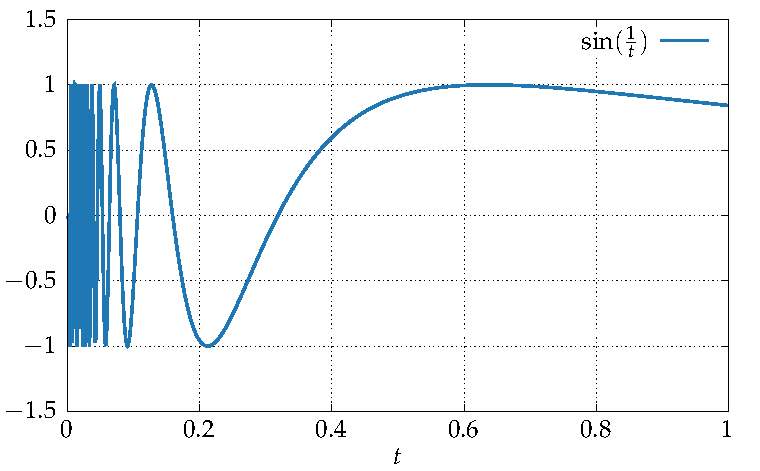
\includegraphics{gp_sininv.pdf}
  \caption{Curve of the function $f(t)=\sin(\frac{1}{t})$ from~\cref{ex:sininv}.}
  \label{fig:sininv}
\end{figure}
Finally, we show that for piecewise smooth functions the one-sided limits of the derivative
can be calculated with the usual limit:
\begin{proposition}
  Let $f$ be a piecewise smooth function on $[a,b]$, and let $t_0\in(a,b)$. The one-sided
  limits of $f'$ are given by the following limits
  \begin{equation}
    f'(t_0^-)=\lim_{\substack{h\to0\\h>0}}\frac{f(t_0)-f(t_0-h)}{h}
    \qquad\text{and}\qquad
    f'(t_0^+)=\lim_{\substack{h\to0\\h>0}}\frac{f(t_0+h)-f(t_0)}{h}
  \end{equation}
\end{proposition}

%%%%%%%%%%%%%%%%%%%%%%%%%%%%%%%%%%%%%%%%%%%%%%%%%%%%%%%%%%%%%%%%%%%%%%%%%%%%%%%%%%%%%%%%%%
\section{Partial Fourier sums}
%.........................................................................................
\subsection{Fourier coefficients}
We start by defining the Fourier coefficients
\begin{definition}
  \label{def:fourier-coef}
  Let $f$ be a piecewise smooth $\tau$-periodic function. We call
  \emph{cosine}, \emph{sine}, and \emph{complex Fourier coefficients} the sequences
  \begin{align}
    a_n(f)&=\frac{2}{\tau}\braket{f,\cw(n\omega)}=\frac{2}{\tau}\int_0^{\tau}\diff t\,f(t)\cos(2\pi n\omega t)\,,\\
    b_n(f)&=\frac{2}{\tau}\braket{f,\sw(n\omega)}=\frac{2}{\tau}\int_0^{\tau}\diff t\,f(t)\sin(2\pi n\omega t)\,,\\
    c_n(f)&=\frac{1}{\tau}\braket{f,\ew(n\omega)}=\frac{1}{\tau}\int_0^{\tau}\diff t\,f(t)\,e^{-2\pi i n\omega t}\,,
  \end{align}
  respectively, where $n\in\mathbb{Z}$ and $\omega=\frac{1}{\tau}$.
\end{definition}
\begin{definition}
  \label{def:fourier-partial}
  Let $f$ be a piecewise smooth $\tau$-periodic function. For any
  integer $N\geq 0$, we call \emph{partial Fourier sum} of degree $N$ the trigonometric
  polynomial defined by
  \begin{equation}
    s_N(f)=\frac{a_0(f)}{2}+\sum_{n=1}^N[a_n(f)\cw(n\omega)+b_n(f)\sw(n\omega)]=
    \sum_{n=-N}^{N}c_n(f)\ew(n\omega)\,,
  \end{equation}
  where $\omega=\frac{1}{\tau}$.
\end{definition}
%.........................................................................................
\subsection{The Riemann-Lebesgue lemma}
\begin{theorem}[Riemann-Lebesgue lemma]
  Let $f$ be a function on $\mathbb{R}$ piecewise smooth on a compact interval
  $[a,b]$. We have the following limit
  \begin{equation}
    \lim_{k\to+\infty}\int_a^b\diff t\, f(t)\sin(kt)=0
  \end{equation}
\end{theorem}
\begin{proof}
  We re-use here the notations of~\cref{def:pw-smooth}. We have
  \begin{equation}
    \int_a^b\diff t\, f(t)\sin(kt)=\sum_{n=0}^{N}\int_{t_n}^{t_{n+1}}\diff t\, f(t)\sin(kt)\,.
    \label{eq:pw-smooth-int}
  \end{equation}
  For a given integer $n$ such that $0\leq n \leq N$, $f$ is continuously differentiable and bounded
  on $(t_n,t_{n+1})$. One can therefore use integration by parts to obtain
  \begin{align}
    \int_{t_n}^{t_{n+1}}\diff t\, f(t)\sin(kt)&=-\frac{1}{k}\left[f(t)\cos(kt)\right]_{t_n}^{t_{n+1}}
    +\frac{1}{k}\int_{t_n}^{t_{n+1}}\diff t\, f'(t)\cos(kt)\notag\\
    &=\frac{1}{k}[f(t_n^+)\cos(kt_n)-f(t_{n+1}^-)\cos(kt_{n+1})]
    +\frac{1}{k}\int_{t_n}^{t_{n+1}}\diff t\, f'(t)\cos(kt)
  \end{align}
  Since $|\cos(kt)|\leq 1$ for all $t\in\mathbb{R}$, the first term in the equation above can be bounded as follows
  \begin{equation}
    \frac{1}{k}|f(t_n^+)\cos(kt_n)-f(t_{n+1}^-)\cos(kt_{n+1})|\leq
    \frac{1}{k}[|f(t_n^+)|+|f(t_{n+1}^-)|]\,,
  \end{equation}
  where we used the triangle inequality $|x+y|<|x|+|y|$. From the inequality above it is
  now clear that
  \begin{equation}
    \lim_{k\to+\infty}\frac{1}{k}\left[f(t)\cos(kt)\right]_{t_n}^{t_{n+1}}=0\,.
  \end{equation}
  Similarly, we have the following inequality
  \begin{equation}
    \frac{1}{k}\left|\int_{t_n}^{t_{n+1}}\diff t\, f'(t)\cos(kt)\right|
    <\frac{1}{k}\int_{t_n}^{t_{n+1}}\diff t\, |f'(t)|\,,
  \end{equation}
  where we use the triangle inequality for integrals $|\int f|<\int |f|$, and we can deduce that
  \begin{equation}
    \lim_{k\to+\infty}\frac{1}{k}\int_{t_n}^{t_{n+1}}\diff t\, f'(t)\cos(kt) =0\,.
  \end{equation}
  In conclusion, we proved that
  \begin{equation}
    \lim_{k\to+\infty}\int_{t_n}^{t_{n+1}}\diff t\, f(t)\sin(kt)=0\,,
  \end{equation}
  which used with~\cref{eq:pw-smooth-int} prove the Riemann-Lebesgue lemma.
\end{proof}
\begin{corollary}
  Let $f$ be a function on $\mathbb{R}$ piecewise smooth on a compact interval
  $[a,b]$. We have the following limits
  \begin{align}
    \lim_{k\to+\infty}\int_a^b\diff t\, f(t)\cos(kt)&=0\,,\\
    \lim_{k\to+\infty}\int_a^b\diff t\, f(t)\,e^{ikt}=0
  \end{align}
\end{corollary}
\begin{corollary}
  Let $f$ be a piecewise smooth $\tau$-periodic function. All the
  Fourier coefficients of $f$ converge to $0$, explicitly
  \begin{equation}
    \lim_{n\to+\infty}a_n(f)=\lim_{n\to+\infty}b_n(f)=\lim_{n\to+\infty}c_n(f)=0\,.
  \end{equation}
\end{corollary}
%.........................................................................................
\subsection{The Dirichlet kernel}
\begin{definition}
  We call~\emph{Dirichlet kernel} of degree $N$ the trigonometric polynomial defined by
  \begin{equation}
    D_N(x)=\sum_{n=-N}^{N}e^{inx}\,,\label{eq:dk-def}
  \end{equation}
  for any real number $x$.
\end{definition}
\begin{proposition}
  \label{prop:dirichlet-id}
  For all $x\in\mathbb{R}$, and all $N\in\mathbb{N}$, we have
  \begin{equation}
    D_N(x)=1+2\sum_{n=1}^{N}\cos(nx)=\frac{\sin[(N+\frac{1}{2})x]}{\sin(\frac{x}{2})}\,.
    \label{eq:dk-sinratio}
  \end{equation}
\end{proposition}
\begin{proof}
  We start by defining the complex number $z$ by
  \begin{equation}
    z=\sum_{n=0}^Ne^{inx}\,.
  \end{equation}
  The Dirichlet kernel can then be written as follows:
  \begin{equation}
    D_N(x)=(z-1)^*+z=z^*+z-1=2\Re(z)-1=1+2\sum_{n=1}^{N}\cos(nx)\,,\label{eq:dk-z}
  \end{equation}
  which proves the first equality in~\cref{eq:dk-sinratio}.
  Since $e^{inx}=(e^{ix})^n$, we can simplify $z$ using a geometric sum:
  \begin{equation}
    z=\frac{e^{i(N+1)x}-1}{e^{ix}-1}\,.\label{eq:dk-geosum}
  \end{equation}
  We now have to compute the real part of $z$, let us start by rewriting the equation above to have a real denominator:
  \begin{equation}
    z=e^{-i\frac{x}{2}}\frac{e^{i(N+1)x}-1}{e^{i\frac{x}{2}}-e^{-i\frac{x}{2}}}
    =\frac{e^{i(N+\frac12)x}-e^{-i\frac{x}{2}}}{2i\sin(\frac{x}{2})}
    =-\frac{i}{2}\frac{e^{i(N+\frac12)x}-e^{-i\frac{x}{2}}}{\sin(\frac{x}{2})}\,,
  \end{equation}
  which has the real part
  \begin{equation}
    \Re(z)=\frac12\frac{\Im[e^{i(N+\frac12)x}]-\Im(e^{-i\frac{x}{2}})}{\sin(\frac{x}{2})}
    =\frac12\frac{\sin[(N+\frac{1}{2})x]}{\sin(\frac{x}{2})}+1\,.
  \end{equation}
  Substituting the last equation into~\cref{eq:dk-z} proves the proposition.
\end{proof}
\begin{proposition}
  The Dirichlet kernel has the following integral on $[0,2\pi]$ for all $N\in\mathbb{N}$:
  \begin{equation}
    \int_0^{2\pi}\diff x\,D_N(x)=2\pi\,.
  \end{equation}
\end{proposition}
\begin{proof}
  Using~\cref{thm:orth-complex} with $m=0$ and $\tau=2\pi$, we obtain
  \begin{equation}
    \int_{0}^{2\pi}\diff x\,e^{inx}=2\pi\,\delta_{n0}\,,
  \end{equation}
  which substituted into~\cref{eq:dk-def} directly proves the proposition.
\end{proof}
\begin{theorem}
  Let $f$ be a piecewise smooth $\tau$-periodic function. For all
  $N\in\mathbb{N}$, the partial Fourier sum has the following integral representation:
  \begin{equation}
    s_N(f)(t)=\frac{1}{\tau}\int_0^{\tau}\diff u\,f(u)\,D_N[2\pi\omega(t-u)]\,.
  \end{equation}
\end{theorem}
\begin{proof}
  Using~\cref{def:fourier-coef,def:fourier-partial}, the partial Fourier sum $s_N(f)$
  is given by
  \begin{equation}
    s_N(f)(t)=\frac{1}{\tau}\sum_{n=-N}^{N}e^{2\pi i n\omega t}
    \int_0^\tau\diff u\,f(u)e^{-2\pi i n\omega u}\,.
  \end{equation}
  Sine the sum above is finite, we can exchange the sum and the integral to obtain
  \begin{equation}
    s_N(f)(t)=\frac{1}{\tau}\int_0^\tau\diff u\,f(u)\sum_{n=-N}^{N}e^{2\pi i n\omega (t-u)}\,.
  \end{equation}
  Finally, using the definition of the Dirichlet kernel~\cref{eq:dk-def} proves the theorem.
\end{proof}
%%%%%%%%%%%%%%%%%%%%%%%%%%%%%%%%%%%%%%%%%%%%%%%%%%%%%%%%%%%%%%%%%%%%%%%%%%%%%%%%%%%%%%%%%%
\section{Convergence of the Fourier expansion}
\subsection{Pointwise convergence}
\begin{theorem}[Fourier]
  \label{thm:fourier-pt}
  Let $f$ be a $\tau$-periodic function which is piecewise smooth on $[0,\tau]$. For all
  $t\in[0,\tau]$, the Fourier series for $f(t)$ converges with the following limit
  \begin{equation}
    \sumz{n}c_n(f)\,e^{2\pi i \omega nt}=\lim_{N\to+\infty}s_N(f)(t)=\frac{f(t^-)+f(t^+)}{2}\,.
  \end{equation}
  In particular, the Fourier series converges to $f(t)$ if $f$ is continuous in $t$.
\end{theorem}
\subsection{Uniform convergence}
\begin{definition}
  A sequence of function $f_n$ is said to \emph{converge uniformly} to $f$ on a domain $D$
  if for all $\epsilon>0$, there exists $N\in\mathbb{N}$ such that
  \begin{equation}
    \forall n\geq N,\quad\forall x\in D,\quad|f_n(x)-f(x)|<\epsilon\,,
  \end{equation}
  which can equivalently be defined as the limit
  \begin{equation}
    \lim_{n\to+\infty}\,\sup_{x\in D}|f_n(x)-f(x)|=0\,.
  \end{equation}
\end{definition}
\begin{theorem}
  Let $f$ be a $\tau$-periodic function which is piecewise smooth and continuous on
  $[0,\tau]$. The Fourier series of $f$ converges uniformly to $f$.
\end{theorem}
\subsection{Gibbs phenomenon}
If a periodic function has a jump discontinuity, then its Fourier series cannot be uniformly
convergent. This generates irregularities around discontinuities where the Fourier expansion tends to ``overshoot'' the function by approximately $9\%$ of the height of the discontinuity. This effect is generally called the \emph{Gibbs phenomenon}, and is a well known engineering issue when cutting data before computing its Fourier coefficients.
A key example of Gibbs phenomenon is the Fourier expansion of the square wave.
\begin{lemma}
  \label{lem:gibbs-sq}
  The square wave Fourier series does not converge uniformly on $[0,1]$, and
  \begin{align}
    \lim_{N\to+\infty}\,s_N(\sq)\left(\frac12-\frac{1}{2N}\right)
    &=1+2\left(\frac{G'}{\pi}-\frac12\right)\,,\label{eq:gibbs-sq-left}\\
    \lim_{N\to+\infty}\,s_N(\sq)\left(\frac12+\frac{1}{2N}\right)
    &=-1-2\left(\frac{G'}{\pi}-\frac12\right)\,,
  \end{align}
  where $G'$ is the \emph{Wilbraham-Gibbs constant} given by
  \begin{equation}
    G'=\int_0^\pi\diff t\,\frac{\sin(t)}{t}\simeq1.851937052\dots\,.
  \end{equation}
\end{lemma}
\begin{proof}
  A guided proof is available as an exercise in Problem~\ref{gibbs}.
\end{proof}
\begin{figure}[t]
  \centering
  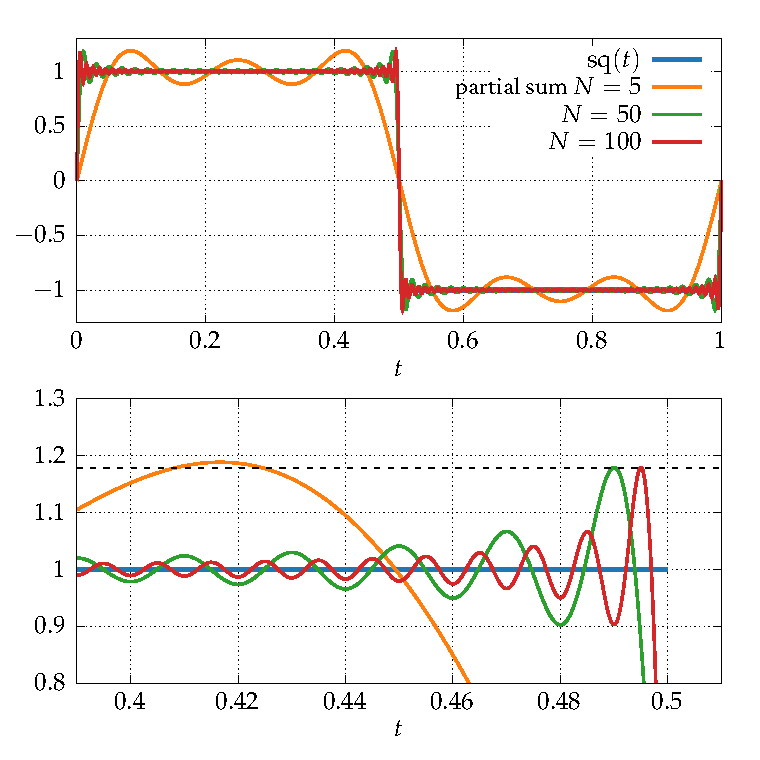
\includegraphics{gp_gibbs-sq.pdf}
  \caption{Gibbs phenomenon in the Fourier expansion of the square wave. The upper pane represents the square wave on one period, and its partial Fourier sum for various degrees. The lower pane is a zoom on the region close to the jump discontinuity at $t=\frac12$, and the dashed line is the excess predicted by~\cref{eq:gibbs-sq-left}.}
  \label{fig:gibbs-sq}
\end{figure}
The Fourier expansion of the square wave is illustrated in~\cref{fig:gibbs-sq}, where the Gibbs phenomenon is clearly visible. The Gibbs phenomenon for the square wave can be generalised to arbitrary discontinuous piecewise smooth functions, as summarised in the theorem below.
\begin{theorem}[Gibbs phenomenon]
  Let be a $\tau$-periodic function which is piecewise smooth on $[0,\tau]$, which has a
  jump discontinuity of height $d$ at $t_0\in(0,\tau)$. Let $[a,b]$ be a sub-interval of
  $[0,\tau]$ such that $t_0\in(a,b)$, and $t_0$ is the only jump discontinuity of $f$ in
  $[a,b]$. The Fourier series of $f$ does not converge uniformly to $f$ on $[a,b]$, and
  \begin{align}
    \lim_{N\to+\infty}\,s_N(f)\left(t_0-\frac{\tau}{2N}\right)
    &=f(t_0^-)-d\left(\frac{G'}{\pi}-\frac12\right)\,,\\
    \lim_{N\to+\infty}\,s_N(f)\left(t_0+\frac{\tau}{2N}\right)
    &=f(t_0^+)+d\left(\frac{G'}{\pi}-\frac12\right)\,,
  \end{align}
  where $G'$ is the Wilbraham-Gibbs constant defined in~\cref{lem:gibbs-sq}.
\end{theorem}
%%%%%%%%%%%%%%%%%%%%%%%%%%%%%%%%%%%%%%%%%%%%%%%%%%%%%%%%%%%%%%%%%%%%%%%%%%%%%%%%%%%%%%%%%%
\section{Properties of Fourier coefficients}
%%%%%%%%%%%%%%%%%%%%%%%%%%%%%%%%%%%%%%%%%%%%%%%%%%%%%%%%%%%%%%%%%%%%%%%%%%%%%%%%%%%%%%%%%%
\section{Multidimensional Fourier series}
